\section{Component Architecture and Design}

\subsection{Design view and component boundaries}

The system architecture in the previous section explains the major runtime blocks. This section refines that view by describing how the application is decomposed into cooperating frontend, backend, persistence, and integration components. The goal of the component design is to keep each major responsibility understandable and testable while still supporting the end-to-end business flow of ordering, administration, kitchen processing, and delivery coordination.

Figure~\ref{fig:component-frontend} and Figure~\ref{fig:component-backend} summarize the main component organization currently reflected in the repository.

\begin{figure}[htbp]
    \centering
    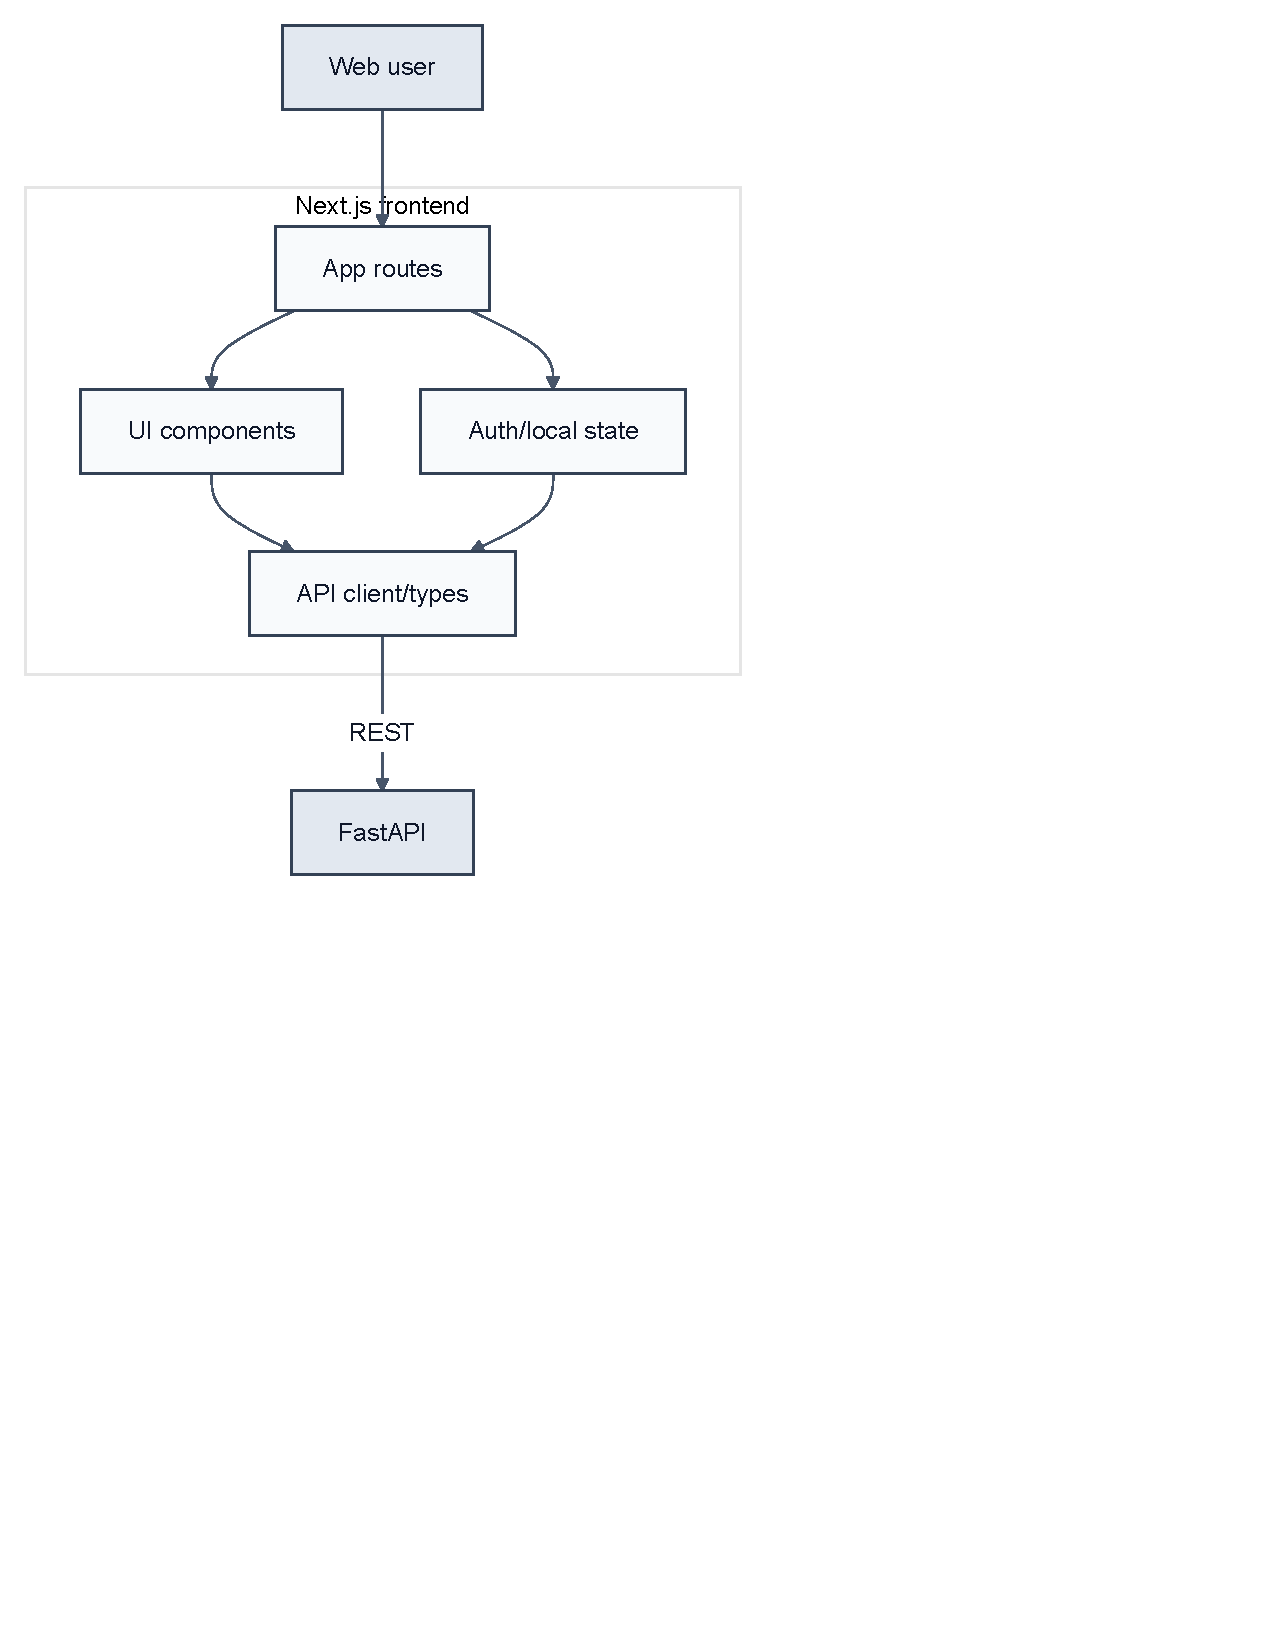
\includegraphics[width=0.78\textwidth,height=0.64\textheight,keepaspectratio,trim=8 367 252 8,clip]{latex_report/figures/component_frontend.pdf}
    \caption{Frontend component architecture}
    \label{fig:component-frontend}
\end{figure}

\begin{figure}[htbp]
    \centering
    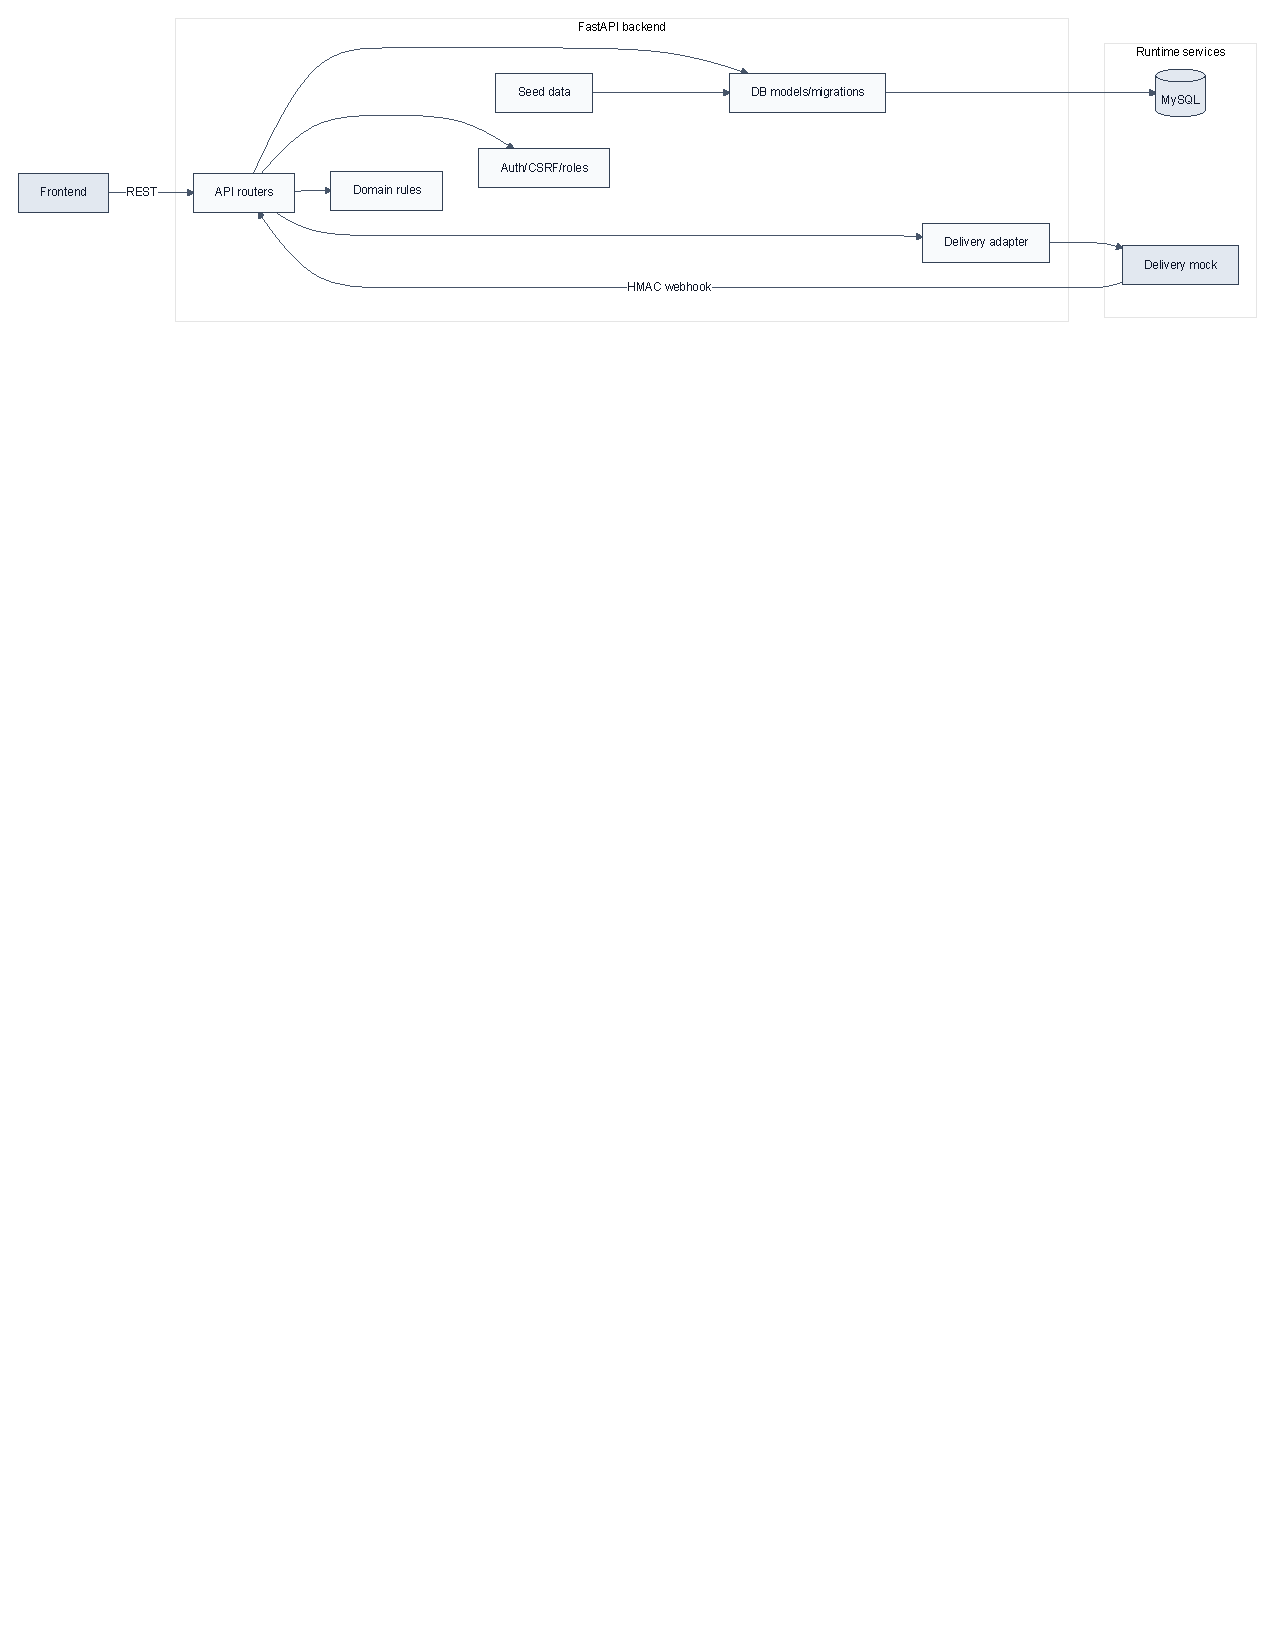
\includegraphics[width=0.95\textwidth,height=0.36\textheight,keepaspectratio,trim=6 632 6 6,clip]{latex_report/figures/component_backend.pdf}
    \caption{Backend and delivery component architecture}
    \label{fig:component-backend}
\end{figure}

\subsection{Frontend component architecture}

The frontend follows a route-plus-components structure centered on the Next.js App Router. Page routes own layout composition and page-level data loading, while reusable UI components encapsulate interaction logic for customer and staff workflows.

\begingroup
\small
\setlength{\LTpre}{0.4em}
\setlength{\LTpost}{0.8em}
\captionof{table}{Frontend component groups}\label{tab:frontend-components}
\begin{tabular}{L{0.19\linewidth} L{0.34\linewidth} L{0.39\linewidth}}
\toprule
\textbf{Component group} & \textbf{Main responsibility} & \textbf{Representative elements} \\
\midrule
Route components & Compose page-level UI, load data, and connect user interaction to feature APIs. & \texttt{app/menu/page.tsx}, \texttt{app/combos/[id]/page.tsx}, \texttt{app/admin/orders/page.tsx}, \texttt{app/kitchen/page.tsx} \\
Public shell components & Provide shared customer-facing navigation, layout chrome, footer, and theme handling. & \texttt{components/app-chrome.tsx}, \texttt{components/top-nav.tsx}, \texttt{components/site-footer.tsx} \\
Menu and product components & Render menu filtering, product cards, option selection, quantity controls, and item-detail UI. & \texttt{components/menu/*} \\
Combo components & Support combo cards, slot picking, step-based combo customization, and quote display. & \texttt{components/combos/*} \\
Administrator components & Support editing, searching, navigation, and management workflows for store operations. & \texttt{components/admin/*} \\
Shared state and auth & Provide session refresh and account-aware UI behavior. & \texttt{components/auth-provider.tsx}, cart provider, theme bootstrap \\
Frontend API layer & Encapsulate fetch behavior, credentials, CSRF injection, typed wrappers, and API error reporting. & \texttt{lib/api/client.ts}, \texttt{lib/api/menu.ts}, \texttt{lib/api/cart.ts}, \texttt{lib/api/admin-*} \\
\bottomrule
\end{tabular}
\endgroup

The frontend is intentionally componentized around business surfaces rather than only around visual primitives. For example, menu customization, combo customization, and administrator editors each have their own specialized component families because they orchestrate different workflow rules even when they share styling conventions.

\subsection{Backend component architecture}

The backend component design mirrors the layered architecture discussed earlier, but it is useful to restate it here in workflow terms.

\begingroup
\small
\setlength{\LTpre}{0.4em}
\setlength{\LTpost}{0.8em}
\captionof{table}{Backend component groups}\label{tab:backend-components}
\begin{tabular}{L{0.19\linewidth} L{0.34\linewidth} L{0.39\linewidth}}
\toprule
\textbf{Component group} & \textbf{Main responsibility} & \textbf{Representative modules} \\
\midrule
Public API routers & Expose catalog browsing, combo browsing, quotation, cart, and order functions. & \texttt{app/api/menu.py}, \texttt{app/api/combos.py}, \texttt{app/api/cart.py}, \texttt{app/api/orders.py} \\
Authentication and account routers & Handle registration, login, session inspection, profile updates, and loyalty access. & \texttt{app/api/auth.py}, \texttt{app/api/loyalty.py}, order-history endpoints \\
Administrative routers & Expose management actions for items, categories, option groups, combos, customers, orders, reports, import, and settings. & \texttt{app/api/admin/*} \\
Kitchen routers & Support kitchen-facing queue inspection and state-changing operational actions. & \texttt{app/api/kitchen/orders.py}, \texttt{app/api/kitchen/actions.py} \\
Integration router & Accept externally initiated delivery callbacks. & \texttt{app/api/webhooks.py} \\
Domain components & Enforce pricing, options, combos, service-area, loyalty, and order-state business logic. & \texttt{app/domain/*} \\
Persistence and support infrastructure & Provide ORM models, DB sessions, migrations, auth helpers, settings access, and delivery-adapter wiring. & \texttt{app/infra/db/*}, \texttt{app/infra/auth/*}, \texttt{app/infra/delivery/*} \\
External-provider simulator & Behave as a realistic network-visible courier system during development and testing. & \texttt{delivery\_mock/main.py} \\
\bottomrule
\end{tabular}
\endgroup

\subsection{Data and integration support components}

Not all important components are visible directly in the UI or API layer. Several supporting components are critical to the overall design:

\begin{itemize}
    \item the SQLAlchemy model layer, which defines durable business state and relationships;
    \item the migration layer, which preserves schema evolution through versioned changes;
    \item the settings service, which centralizes configurable values such as business timezone, loyalty parameters, and delivery fee mapping;
    \item the delivery-port abstraction, which isolates delivery-provider behavior from core order workflows;
    \item the generated OpenAPI contract and TypeScript types, which connect backend response models to frontend usage safely.
\end{itemize}

These support components are important because they reduce duplication of business rules and make cross-layer behavior more consistent.

\subsection{Component interaction scenarios}

\subsubsection{Pizza quotation flow}

When a customer opens an item-detail page, the route component loads product information and exposes option-selection controls through menu components. User choices are then packaged by the frontend API layer and sent to the quotation endpoint. On the backend, the cart quote router resolves the current product and enabled options from persistence, validates the selection through the options domain, and calculates totals through the pricing domain before returning an authoritative quote.

\subsubsection{Combo customization flow}

Combo customization involves a richer interaction path. The frontend combo customizer presents fixed components and category-scoped choice slots. The backend resolves combo definitions, validates slot selections, calculates any surcharge relative to the slot reference product, and combines that with option-delta pricing. This scenario shows why combo-related logic is not just a variant of simple product pricing.

\subsubsection{Administrative combo editing flow}

In the administrative interface, a combo editor page coordinates multiple component families: basic form controls, component pickers, image handling, and API mutation calls. The backend administrative combo router validates date ranges, component structure, and category-slot constraints before persistence. This interaction demonstrates how the system separates staff-facing CRUD orchestration from reusable domain rules.

\subsubsection{Delivery callback flow}

The delivery callback flow crosses the clearest system boundary. The delivery mock sends an HMAC-signed HTTP callback to the webhook router. The backend verifies the signature, enforces idempotency, maps the provider event to an internal order-state transition, and records a tracking entry. This scenario shows how integration logic, domain rules, persistence, and workflow history cooperate without requiring direct user interaction.

\subsection{Design rationale}

The component design of PizzaHUST follows three consistent principles:

\begin{itemize}
    \item \textbf{business-oriented decomposition:} components are grouped around meaningful workflows such as customization, administration, kitchen actions, and delivery integration;
    \item \textbf{separation of orchestration from rules:} routers and pages coordinate actions, while domain modules enforce reusable business logic;
    \item \textbf{support for incremental delivery:} the design allows some components to be implemented or refined earlier than others without collapsing the whole structure.
\end{itemize}

The current codebase is not perfectly uniform in every frontend data-access pattern, especially in some administrative pages, but the dominant structure is consistent enough to support maintainability and verification. For the scope of an academic project, this is a sound component design outcome.
